\documentclass{bredelebeamer}

% Customs:
\usepackage[utf8]{inputenc}
\usepackage{amsmath,amsfonts,amssymb,graphicx}
\usepackage[document]{ragged2e}
\usepackage[Euler]{upgreek}

% Define mathbfit
\DeclareMathAlphabet{\mathbfit}{OML}{cmm}{b}{it}
\DeclareMathAlphabet{\mathbfsf}{\encodingdefault}{\sfdefault}{bx}{n}

\usepackage[backend=biber]{biblatex}
\addbibresource{ref.bib}

% Setting graphics path
\graphicspath{{./rsc/}{./rsc/pdf/}{./rsc/svg/}{./rsc/image/}}

% Define operators
\DeclareMathOperator*{\argmax}{arg\,max}
\DeclareMathOperator*{\argmin}{arg\,min}

% Define textbfit
\makeatletter
\DeclareRobustCommand\bfseriesitshape{
  \not@math@alphabet\itshapebfseries\relax
  \fontseries\bfdefault
  \fontshape\itdefault
  \selectfont
}
\makeatother
\DeclareTextFontCommand{\textbfit}{\bfseriesitshape}

\usefonttheme[onlymath]{serif}

%%%%%%%%%%%%%%%%%%%%%%%%%%%%%%%%%%%%%%%%%%%%%%%% META DATA start

\title[ML Basics]{Machine Learning Basics}
% Titre du diaporama

\subtitle{A self-study metarials for PRML~\cite{bishop:2006:PRML}}
% Sous-titre optionnel

\author{Jisung Lim\inst{1}}
% The \inst {...} command displays the member's affiliation.
% If there are several speakers: Marcel Dupont \inst {1}, Roger Durand
% \inst {2} Simply add another institute on the model below.

\institute[ML studio]
{
  \inst{1}%
  B.S. Candidate of Industrial Engineering\\
  Yonsei University, South Korea.
}

\date{28th January, 2017}
% Optional. The date, usually the day of the conference.

\subject{Basic-level study metarials for machine learning.}
% This is used in the pdf metadata

\logo{
  \begin{tikzpicture}
    \pgfmathsetmacro{\myopacity}{0.25}
    \node[opacity=\myopacity] {
      
\includegraphics[scale=0.08]{yonsei_emblem.png}
      
\includegraphics[scale=0.08]{yonsei_logo_text.png}
    };
  \end{tikzpicture}
}

%%%%%%%%%%%%%%%%%%%%%%%%%%%%%%%%%%%%%%%%%%%%%%%% META DATA end

%%%%%%%%%%%%%%%%%%%%%%%%%%%%%%%%%%%%%%%%%%%%%%%% DOCUMENT start

\begin{document}

%%%%%%%%%%%%%%%%%%%%%%%%%%%%%%%%%%%%%%%%%%%%%%%%%%%%%%%%%%% TITLE PAGE

\begin{frame}
  \titlepage
\end{frame}

%%%%%%%%%%%%%%%%%%%%%%%%%%%%%%%%%%%%%%%%%%%%%%%%%%%%%%%%%%% SUMMARY

\begin{frame}{Summary}
  \tableofcontents
  % Option to add option [pausesections]
\end{frame}

%%%%%%%%%%%%%%%%%%%%%%%%%%%%%%%%%%%%%%%%%%%%%%%%%%%%%%%%%%%%%%%%%%%%%

\section{Introduction}
\subsection{How to solve complex problem?}
\begin{frame}{Optical Character Recognition}
  \textbf{OCR Problem and Some Approaches}
  \begin{columns}
    \begin{column}{0.3\textwidth}
      \begin{figure}
      \centering
      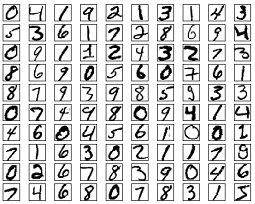
\includegraphics[scale=0.5]{mnist_pic.png}
      \caption{
        \href{https://en.wikipedia.org/wiki/MNIST_database}{The MNIST database}.
      }
      \end{figure}
    \end{column}
    \begin{column}{0.7\textwidth}
      \begin{itemize}
        \item \textbf{Input}: ${28}\times{28}$ pixel image, represented by
              a vector $\mathbfit{x}$ comprising $784$ real numbers.
        \item \textbf{Goal}: To build a machine that will take such
              a vector $\mathbfit{x}$ as input and that will produce
              the identity of the digit $0,\ldots,9$ as the output.
      \end{itemize}
    \end{column}
  \end{columns}
  Consider the example of recognizing handwritten digits, illustrated in Figure
  1. This is the nontrivial problem due to the wide variability of handwriting.
  And we can tackle this problem using following approches:
  \begin{enumerate}
    \item Handcrafted rules or heuristics
    \item Machine learning methods
  \end{enumerate}
  In practice, the former leads to a proliferation of rules
  and invariably gives poor results. For better results, the
  latter can be considered an alternative.
\end{frame}

\subsection{What is machine learning?}
\begin{frame}{Machine Learning Approach}
  \begin{justify}
    \textbf{Machine Learning Approach} can be divided into three major stages:
    \textbf{training}, \textbf{testing}, and \textbf{predicting}. The overall
    process of a machine learning approach to classification problems such as
    OCR can be depicted in Figure 2.
  \end{justify}
  \begin{figure}[h]
  \centering
  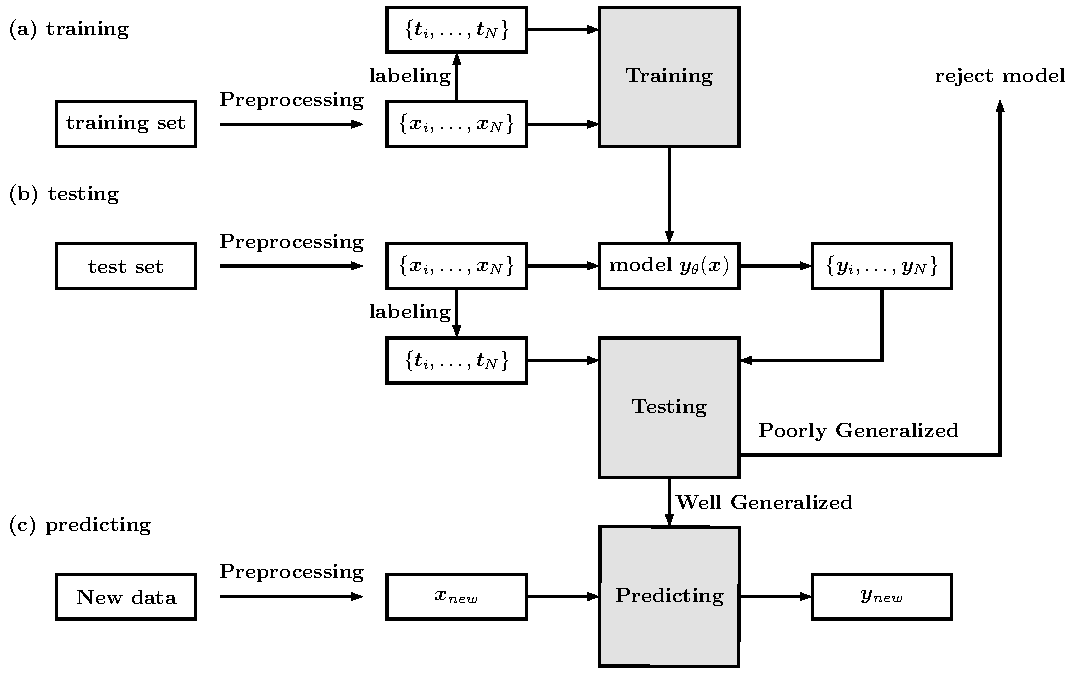
\includegraphics[scale=0.45]{desc_ml_approach.pdf}
  \caption{
    The overall process of machine learning approach, especially of supervised learning.
  }
  \end{figure}
\end{frame}

\begin{frame}{ML Approach --- Input}
  \begin{justify}
    First of all, we need to define inputs more precisely. In OCR, inputs are
    handwriting images of a digit. In practical applications, the original input
    images may have different sizes, ratios, angles, or even colors. Hence, the
    images are typically scaled, rotated, translated, and grey-scaled so that
    each digit is contained within a box of a fixed-size, says $28 \times 28$,
    and is toned with greyscale color. And then, the preprocessed input images
    can be represented as a vector $\mathbfit{x}=(x_{1},\ldots,x_{784}) \in
    \mathbb{R}^n$ where the greyscale color of $i$th pixel is a $x_i$. Finally,
    you should label the true number $\mathbfit{t}$ for each input image
    $\mathbfit{x}$.
  \end{justify}
  \begin{columns}
    \begin{column}{0.1\textwidth}
      \begin{figure}[h]
      \centering
      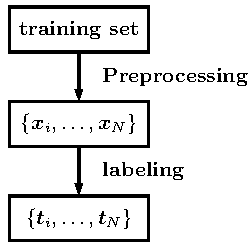
\includegraphics[scale=0.5]{desc_input.pdf}
      \caption{ }
      \end{figure}
    \end{column}
      \begin{column}{0.8\textwidth}
        \begin{description}
          \item [\textbf{Preprocess}:]
            \begin{justify}
              To transform the original input variables into some new space
              of variables so that the problem becomes easier to solve.
            \end{justify}
          \item [\textbf{Example} $\mathbfit{x}_i$:]
            \begin{justify}
              An example is a collection of features. Typically, an
              \textbf{example} will be represented as a vector
              $\mathbfit{x}_i \in \mathbb{R}^n$ where each entry $x_i$ is a
              \textbf{feature}.
            \end{justify}
          \item [\textbf{Label} $\mathbfit{t}_i$:]
            \begin{justify}
              A \textbf{label} represents the identity of the corresponding
              digit. Typically, the labels are hand-labelled by inspecting
              each image individually. Note that there is one such
              \textbf{label} $\mathbfit{t}_i$ for each \textbf{example}
              $\mathbfit{x}_i$.
            \end{justify}
        \end{description}
      \end{column}
  \end{columns}
\end{frame}

\begin{frame}{ML Approach --- Train and Test}
  \begin{columns}
    \begin{column}{0.4\textwidth}
      \begin{figure}[h]
      \centering
      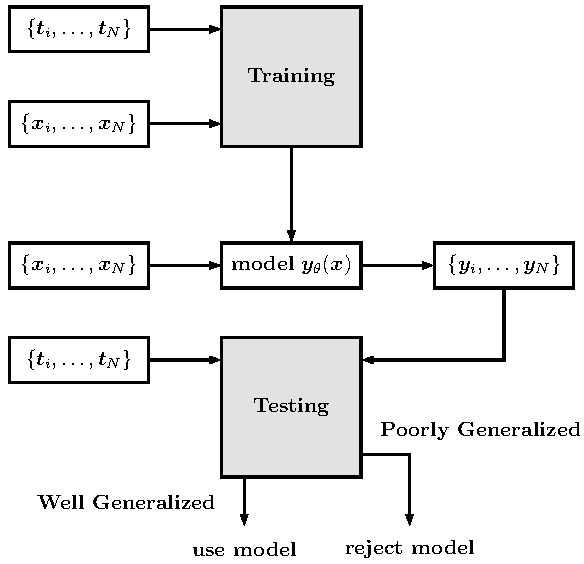
\includegraphics[scale=0.5]{desc_training_test.pdf}
      \caption{
        The description of training and test.
      }
      \end{figure}
    \end{column}
    \begin{column}{0.6\textwidth}
      \begin{itemize}
        \item \textbf{Training} \\
        \begin{justify}
          To tune the parameters of an adaptive model, it uses a large set of $N$
          \textbf{examples} $\{\mathbfit{x}_1,\ldots,\mathbfit{x}_N\}$ with its
          corresponding \textbf{labels} $\{\mathbfit{t}_1,\ldots,\mathbfit{t}_N\}$.
          The model can be expressed as a function $\mathbfit{y(x)}$ which takes
          a new digit image $\mathbfit{x}_{new}$ as input and that generates an
          output vector $\mathbfit{y}_{new}$.
        \end{justify}
        \item \textbf{Testing} \\
        \begin{justify}
          Once the model is trained it can then determine the identity of new
          digit images, which are said to comprise a test set. The ability to
          categorize correctily new examples that differ from those used for
          training is known as \textbf{generalization}. In practical
          applications, the variability of the input vectors will be such that
          the training data can comprise only a tiny fraction of all possible
          input vectors, and so generalization is a central goal in pattern
          recognition.
        \end{justify}
      \end{itemize}
    \end{column}
  \end{columns}
\end{frame}

\begin{frame}{ML Approach --- Prediction model}
  \begin{justify}
    Let's go back to handwriting recognition. First, the key to the handwriting
    recognition problem is to classify entirely new, unseen data into the
    appropriate class. In particular, machine learning methods learn and test
    through preprocessed (labeled) data as we have seen so far to generate a
    predictive model. Since, through the testing stage, the prediction model has
    been verified to be sufficiently generalized, it can respond appropriately
    to new data and can be described as follows.
  \end{justify}
  \begin{figure}[h]
  \centering
  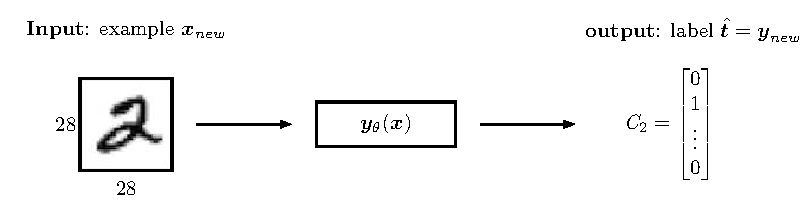
\includegraphics[scale=0.8]{ocr_ml_desc.pdf}
  \caption{The description of prediction in OCR.}
  \end{figure}
\end{frame}

\begin{frame}{ML Approach --- SL, UL, and RL}
  \begin{itemize}
    \item[SL]
    \begin{justify}
      \textbf{Supervised Learning}:\\
      Supervised learning is the machine learning task of inferring a function
      from labeled training data~\cite{Mohri:2012:FML:2371238}. The \textbf{data}
      consists of a set of examples, each of which is \textit{a pair of an input
      value and corresponding desired output value}.\\
      Ex. Regression, Classification.
    \end{justify}

    \item[UL]
    \begin{justify}
      \textbf{Unsupervised Learning}:\\
      Unsupervised learning is the machine learning task of inferring a function
      to describe hidden structure from unlabeled data. Since the examples given
      to the learner are unlabeled, there is no error or reward signal to
      evaluate a potential solution – this distinguishes unsupervised learning
      from supervised learning and reinforcement learning.\\
      Ex. Clustering, Density estimation.
    \end{justify}

    \item[RL]
    \begin{justify}
      \textbf{Reinforcement Learning}:\\
      A goal of reinforcement learning is \textbf{to find an action} which gives
      \textbf{greatest reward} by \textbf{interacting with a given environment}.
      It discovers the optimal by a process of \textbf{exploration and exploitation}.
      (A reinforcement learning agent interacts with its environment in discrete
      time steps. At each time $t$, the agent tries to find a suitable action
      $a_{t}$ which moves the current environment $s_{t}$ to next state $s_{t+1}$
      and determines a corresponding reward $r_{t+1}$. It discovers the optimal
      action by balancing the trade-off between \textbf{exploration}, in whcih
      the system \textbf{tries out new kinds of actions} to see how effective
      they are, and \textbf{exploitation}, in which the system \textbf{makes
      use of actions} that are known to yield a high reward.)
    \end{justify}
  \end{itemize}
\end{frame}

\begin{frame}{Precise Definition of ML}
  \begin{block}{Definition of machine learning}
    A computer program is said to \textbfit{learn}
    from \textbf{experience} \textbfit{E}
    with respect to some class of \textbf{tasks} \textbfit{T}
    and \textbf{performance measure} \textbfit{P},
    if its performance at tasks in \textbfit{T},
    as measured by \textbfit{P},
    improves with experience \textbfit{E}.
  \end{block}
\end{frame}

\section{Polynomial Curve Fitting}
\subsection{Polynomial curve fitting}
\begin{frame}{Polynomial Curve Fitting}
  \textbf{Given Situation}
  \begin{itemize}
    \item $N$ labeled observations.

  \end{itemize}
  \begin{itemize}
    \item\begin{justify}
      $N$ observations $\mathbfsf{X} \equiv {(x_1,\ldots,x_N)}^{T}$, together
      with corresponding labels $\mathbfsf{t} \equiv {(t_1,\ldots,t_N)}^{T}$
    \end{justify}
    \item\begin{justify}
      $(\mathit{x}_i, \mathit{t}_i)$ possess underlying regularity, which
      we wish to learn.
    \end{justify}
    \item\begin{justify}
      Individual $\mathit{t}_i$ observations are corrupted by random noise,
      which might arise from intrinsical stochasticity due to there being
      source of variability.
    \end{justify}
  \end{itemize}

  \textbf{Our Goal and Intrinsic Difficulty}
  \begin{itemize}
    \item\begin{justify}
      \textbf{Goal}: To exploit this given training set in order to make
      prediction of the value $\hat{t}$ of the target variable for some new
      value $\hat{x}$ of the input variable.
    \end{justify}
    \item\begin{justify}
      \textbf{Intrinsic Difficulty}: This is a intrinsically difficult problem
      not only as we have to generalize from a \textbf{finite data} set but also,
      for a given $\hat{x}$ there is \textbf{uncertainty} as to the appropriate
      value for $\hat{t}$.
    \end{justify}
  \end{itemize}
\end{frame}

\begin{frame}{Polynomial Function as a Estimate $\hat{t}=y(\mathit{x},\mathbfit{w})$}
  \begin{justify}
    Consider a simple approach based on curve fitting. We can use the polynomial
    function to fit the data. The value $\hat{t}=y(\mathit{x},\mathbfit{w})$ of
    the function is an estimate of the target value $t$.
    \begin{equation}
      \hat{t} = y(\mathit{x}, \mathbfit{w}) = \sum_{j=0}^{M} {{w_j}{x^j}}
    \end{equation}
    \begin{itemize}
      \item Since $M$ is the order of the polynomial, determining $M$ has meaning
      as a \textbf{model selection}. Model selection generally makes a big difference
      in fitting performance and should be considered separately from the modeling data.
      \item The values of the coefficients $w_j$ will be determined by \textbf{fitting}
      the polynomial to the training data. This can be done by minimizing difference
      between the target value $t$ and and its estimate $\hat{t}=y(\mathit{x},\mathbfit{w})$.
    \end{itemize}
  \end{justify}

\end{frame}

\begin{frame}{Error Minimization}
  \begin{justify}
    We first define an error function $E(\mathbfit{w})$ that serve as a criteria
    for not only how to select the best model based on training data but also how
    well the model fits into the test data. We can use sum of squared errors as a
    error function.
    \begin{equation}
      E(\mathbfit{w}) = \frac{1}{2}\sum_{n=1}^{N} { \{ y(\mathit{x}_\mathit{n},\mathbfit{w})-\mathbfit{t}_\mathit{n} \} }^{2}
      \quad \textrm{where} \quad y(\mathit{x}, \mathbfit{w})=\sum_{\mathit{j}=0}^{\mathit{M}} {{\mathit{w_j}}{\mathit{x^j}}}
    \end{equation}

    You can also use root mean square to validate the model with the test set.
    \begin{equation}
      E_{RMS}(\mathbfit{w}^{*}) = \sqrt{ {2} E(\mathbfit{w}^{*}) / {N} }
    \end{equation}
    RMS has two advantages as followings:
    \begin{enumerate}
      \item $\mathbfit{1/N}$ Normalize the size of the data set, so that it makes
            possible to compare different sizes of data sets on an equal footing.
      \item $\sqrt{E(\cdot)}$ Remove square property of $E(\mathbfit{w})$ so that
            this ensures the same measure scale between error function $E_{RMS}$
            and target value $\mathit{t}$.

    \end{enumerate}
  \end{justify}
\end{frame}

\begin{frame}{Regularization}
  \begin{justify}
    Add regularization term to error function $E(\mathbfit{w})$ for preventing
    overfitting.
    \begin{equation}
      \tilde{E}(\mathbfit{w})=E(\mathbfit{w})+\frac{\lambda}{2}\mathbfit{w}^{T}\mathbfit{w}
    \end{equation}

    The coefficient $\lambda$ governs the relative importance of the
    regularization term.
    \begin{equation}
      \ln\lambda=\left\{\begin{aligned}
        & {-\infty} \quad && (\lambda\rightarrow0) \quad && \text{(overfitting)}  \\
        & {K}       \quad && (0<\lambda<1)         \quad && \text{(well fit)}     \\
        & {0}       \quad && (\lambda=1)           \quad && \text{(underfitting)}
      \end{aligned}\right.
    \end{equation}
  \end{justify}
\end{frame}

\begin{frame}{Hyperparameter}
  \begin{itemize}
    \item\begin{justify}
    \textbf{Hyperparameter} \\
    Hyperparameter is a parameter that controls the complexity of machine learning
    model. In polynomial curve fitting problem, the order of polynomial $M$ and the
    coefficient $\lambda$ which governs the relative importance of the regularizer
    are hyperparameters. Sometimes we can optimize or learn it, but most of time it
    is not appropriate to learn that hyperparameter on the training set.
    \end{justify}
    \item\begin{justify}
    \textbf{Validation set} \\
    To solve above problem, we need a validation set of examples which is separately
    obtained from either training or test set. In polynomial curve fitting problem,
    by taking the available data and partitioning it into a \textbf{training set},
    used to determine the coefficients $\mathbfit{w}$, and a separate
    \textbf{validation set}, also called a hold-out set, used to optimize the model
    complexity (either $M$ or $\lambda$).
    \end{justify}
  \end{itemize}
\end{frame}

\subsection{Chapter objectives}
\begin{frame}{Chapter Objectives}
  \begin{itemize}
    \item \begin{justify}
      \textbf{Probability Theory}\\
      provides a consistent framework for expressing an uncertainities in a
      precise and quantitative manner. \\
      \textbf{Keywords.}
      Two rules of probability (sum rule and product rule), Random variable,
      Probabilty mass and density, Frequentist vs. Bayesian, Estimation (MLE, MAP),
      Bias, Full Bayesian process (bayesian prediction).
    \end{justify}
    \item\begin{justify}
      \textbf{Decision Theory}\\
      allows us to exploit this probabilistic representation to make optimal
      prediction according to appropriate criteria. \\
      \textbf{Keywords.}
      Inference stage and decision stage, Loss function, Reject option,
      Gen or Dis, Usefulness of a posterior \\
      \textbf{Additionals.}
      Functional, Calculus of Variations, Lagrangian and KKT conditions \\
    \end{justify}
    \item\begin{justify}
      \textbf{Information Theory} \\
      describes, in terms of amount of information, how to encode a random event,
      calculate the average amount of information in a random variable, and compare
      two different distributions. \\
      \textbf{Keywords.}
      Self information and joint, conditional, or mutual information,
      Entrophy and differential entrophy, Maximum entrophy, KL divergence.
    \end{justify}
  \end{itemize}

\end{frame}

%%%%%%%%%%%%%%%%%%%%%%%%%%%%%%%%%%%%%%%%%%%%%%%%%%%%%%%%%%%%%%%%%%%%%

\section{Probability Theory}
\subsection{Probability Basic}
\begin{frame}{Where the uncertainty comes from?}
  \begin{itemize}
    \item\begin{justify}
      \textbf{Inherent stochasticity}\\
      A system could contains intrinsic random factors, so we should take those
      factors into account to design a model.\\
      e.g. Shuffle in card game, Customers or accidents come randomly
    \end{justify}
    \item\begin{justify}
      \textbf{Incomplete observability}\\
      Sometimes, the system cannot be fully observed. Even if the outcome is
      deterministic, it might be considered a stochastic system if the outcome is
      not known exactly.\\
      e.g. Monty Hall Game, Bayesian Statistics
    \end{justify}
    \item\begin{justify}
      \textbf{Incomplete modeling}\\
      To simplify, we can ignore information we already know. In this case, the
      information can be treated as stochastic. Sometimes, simple stochasticity
      is much better than complex deterministicity.\\
      e.g. Discretize space for robot.
    \end{justify}
  \end{itemize}
\end{frame}

\begin{frame}{Random Variable}
  \begin{itemize}
    \item\begin{justify}
      \textbf{Random Experiment}\\
      An experiment whose outcome cannot be predicted with certainty before the
      experiment is excuted. In classical or frequency-based probability theory,
      we also assume that the experiment can be repeated indefinitely under
      essentially the same conditions (e.g. Bernoulli trial). The repeatability
      assumption is important because the classical theory is concerned with the
      long-term behavior as the experiment is replicated. By contrast, subjective
      or belief-based probability theory is concerned with measures of belief
      about what will happen when we run the experiment. In this view, repeatability
      is a less crucial assumption.
    \end{justify}
    \item\begin{justify}
      \textbf{Sample Space}\\
      The sample space of a random experiment is a set $S$ that includes all
      possible outcomes of the experiment; the sample space plays the role of the
      universal set when modeling the experiment.
    \end{justify}
    \item\begin{justify}
      \textbf{Events}\\
      Certain subsets of the sample space of an experiment are referred to as events.
    \end{justify}
  \end{itemize}
\end{frame}

\begin{frame}{Random Variable (conti\ldots)}
  \begin{itemize}
    \item\begin{justify}
      \textbf{Random Variable}\\
      Suppose again that we have a random experiment with sample space $S$.
      A mapping $\mathrm{x}$ from $S$ into another set $T$ is called a ($T$-valued)
      random variable. If sample sapce is a countable set, then we call this
      random variable $\mathit{discrete}$. If an uncountable set, then $\mathit{continuous}$.
    \end{justify}
    \item\begin{justify}
      \textbf{Probability Measure}\\
      A probability measure (or probability distribution) $\mathbb{P}$ for a
      random experiment is a real-valued function, defined on the collection of
      events, that satisfies the following axioms:
      \begin{enumerate}
        \item $\mathbb{P}(A) \geq 0$ for every event $A$
        \item $\mathbb{P}(S) = 1$
        \item If $A_i : i \in I$ is countable, pairwise disjoint collection of events, then
        \begin{equation}
          \mathbb{P}(\cup_{i \in I} A_i) = \sum_{i \in I} \mathbb{P}(A_i)
        \end{equation}
      \end{enumerate}
    \end{justify}
  \end{itemize}
\end{frame}

\begin{frame}{Probability Density Function}
  \begin{itemize}
    \item\begin{justify}
      \textbf{Probability Density Function}\\
      If $\mathrm{x}$ is a random variable, the probability density functyion of
      $\mathrm{x}$ is the function $p(\mathrm{x}=\mathit{x})$ on $S$ that assigns
      probabilities $p$ to the point $\mathrm{x}=\mathit{x}$ in $S$:
      \begin{enumerate}
        \item $p(\mathit{x}) \geq 0, \forall \mathit{x} \in S$
        \item $\int_S p(\mathit{x})\, \mathrm{dx} = 1$
        \item $\int_A p(\mathit{x})\, \mathrm{dx} = \mathbb{P}(\mathrm{x} \in A), \forall A \subseteq S$
      \end{enumerate}
    \end{justify}
    \item\begin{justify}
      \textbf{Probability Distribution}\\
      A probability distribution $p(\mathrm{x}=\mathit{x})$ of random variable
      $\mathrm{x}$ is the function that assigns probabilities to the subset of
      $S$, namely:
      \begin{equation}
        A \mapsto \mathbb{P}(\mathrm{x} \in A) \  \textrm{for} \  A \subseteq S
      \end{equation}
      If we use parametrized distribution, then we can use the notation such as:
      \begin{equation}
        \mathrm{x} \sim U(\mathit{x}; \alpha, \beta)
      \end{equation}
    \end{justify}
  \end{itemize}
\end{frame}

\begin{frame}{Basic Rules}
  For convenience, we will use more simple notation $\mathbb{P}(A)$ instead of
  $\mathbb{P}(\mathrm{x} \in A)$.
  \begin{itemize}
    \item\textbf{Sum Rule}
    \begin{equation}
      \mathbb{P}(A+B)=\mathbb{P}(A)+\mathbb{P}(B)-\mathbb{P}(A \cap B)
    \end{equation}
    \item\textbf{Product Rule}
    \begin{equation}
      \mathbb{P}(A \cap B)=\mathbb{P}(A|B)\mathbb{P}(B)=\mathbb{P}(B|A)\mathbb{P}(A)
    \end{equation}
    \item\textbf{Chain Rule}\\
    By product rule with recursive manner, we get
    \begin{equation}
      \mathbb{P}(X_{0 : N-1})=\mathbb{P}(X_0)\mathbb{P}(X_1|X_0)\cdots\mathbb{P}(X_{N-1}|X_{0 : N-2})
    \end{equation}
    \item\textbf{Marginal Probability}
    \begin{equation}
      \mathbb{P}(A) = \int_A p(x)\, \mathrm{dx}
      = \int_A \int_Y p(x,y)\, \mathrm{dy}\mathrm{dx}
    \end{equation}
    \item\textbf{Conditional Probability}
    \begin{equation}
      \mathbb{P}(A|x) = \int_A p(y|x)\, \mathrm{dy}
                      = \int_A \frac{p(x, y)}{p(x)}\, \mathrm{dy}
                      = \int_A \frac{p(x, y)}{\int_Y p(x,y)\, \mathrm{dy}}\, \mathrm{dy}
    \end{equation}
  \end{itemize}
\end{frame}

\begin{frame}{Bayes Rule}
  \begin{itemize}
    \item\begin{justify}
      \textbf{Bayes Rule}\\
      By conditional probability, we get bayes rule
      \begin{equation}
        \mathbb{P}(A|B) = \frac{\mathbb{P}(A, B)}{\mathbb{P}(A)}
        = \frac{\mathbb{P}(A, B)}{\int_{Y} \mathbb{P}(A,B)\, \mathrm{d}y}
      \end{equation}
    \end{justify}
    \item\begin{justify}
      \textbf{In the perspective of machine learning}\\
      We may substitute $x$ and $y$ for $H$, which denotes a model hypothesis,
      and $D$, which denotes a data set.
      \begin{equation}
        \mathbb{P}(H|D)
          = \frac{\mathbb{P}(H,D)}{\mathbb{P}(D)}
          = \frac{\mathbb{P}(H,D)}{\sum_H \mathbb{P}(H,D)}
          = \frac{\mathbb{P}(H)\mathbb{P}(D|H)}{\sum_H \mathbb{P}(H)\mathbb{P}(D|H)}
      \end{equation}
      We call $\mathbb{P}(H)$ prior, $\mathbb{P}(H|D)$ posterior,
      $\mathbb{P}(D|H)$ likelihood, and $\mathbb{P}(D)$ evidence.
    \end{justify}

  \end{itemize}
\end{frame}

%\begin{frame}{Transformation of density function}

%\end{frame}

\begin{frame}{Independence}
  \begin{itemize}
    \item\begin{justify}
      \textbf{Independence}\\
      We says random variable $\mathrm{x}$ and $\mathrm{y}$ are independence if
      \begin{equation}
        p(x,y) = p(x)p(y), \forall x \in \mathrm{x}, y \in \mathrm{y}
      \end{equation}
      This also means that $p(x) = p(x|y), p(y) = p(y|x), \forall x \in \mathrm{x}, y \in \mathrm{y}$.
      We denotes independence between $\mathrm{x}$ and $\mathrm{y}$ into $\mathrm{x}\perp\mathrm{y}$.
    \end{justify}
    \item\begin{justify}
      \textbf{Conditionally Independence}\\
      We says random variable $\mathrm{x}$ and $\mathrm{y}$ are conditionally
      independence given $\mathrm{z}$, if there exist function $g$ and $h$ such that
      \begin{equation}
        p(x,y|z) = g(x,z)h(y,z), \forall x \in \mathrm{x}, y \in \mathrm{y}, z \in \mathrm{z}
      \end{equation}
      We denotes conditionally independence between $\mathrm{x}$ and $\mathrm{y}$
      given $\mathrm{z}$ into $\mathrm{x}\perp\mathrm{y}\,|\,\mathrm{z}$.
    \end{justify}
  \end{itemize}
\end{frame}

\begin{frame}{Expactation and Variance}
  \begin{itemize}
    \item\begin{justify}
      \textbf{Expectation}\\
      Expectation means expected value of $f(x)$ when $x$ is drawn from $P(\mathrm{x}=x)$.
      We can get expectation of $f(x)$ by
      \begin{equation}
        \mathbb{E}_{\mathrm{x} \sim P} [f(x)] = \int_\mathrm{x} f(x)P(\mathrm{x}=x)\,\mathrm{dx}
      \end{equation}
      Expectations are linear functional,
      \begin{equation}
        \mathbb{E}_{\mathrm{x} \sim P} [\alpha f(x) + \beta g(x)]
          = \alpha \mathbb{E}_{\mathrm{x} \sim P} [f(x)] + \beta \mathbb{E}_{\mathrm{x} \sim P} [g(x)]
      \end{equation}
    \end{justify}
    \item\begin{justify}
    \textbf{Variance}\\
    Variance means how much the values of a function of a random variable
    $\mathrm{x}$ vary as we sample different values of $\mathrm{x}$ from its
    distribution:
    \begin{equation}
      \mathit{Var}_{\mathrm{x} \sim P} [f(x)] = \mathbb{E}_{\mathrm{x} \sim P} [\{ f(x) - \mathbb{E}[f(x)] \} ^2]
    \end{equation}
    The square root of the variation called $\mathit{standard\ deviation}$.\\
    \end{justify}
    \item\begin{justify}
    \textbf{Covariance}\\
    Covariance gives information about how two values are linearly related, as well as
    the scale of these variables:
    \begin{equation}
      \mathit{Cov}_{\mathrm{x}, \mathrm{y}} [f(x), g(y)]
      = \mathbb{E}_{\mathrm{x}, \mathrm{y}} [\{ f(x) - \mathbb{E}_{\mathrm{x}}[f(x)] \} \{ g(y) - \mathbb{E}_{\mathrm{y}}[g(y)] \} ^T]
    \end{equation}
    \end{justify}
  \end{itemize}
\end{frame}

\subsection{Bayesian and degree of belief}
\begin{frame}{Frequentist vs Bayesian}
  \textbfit{Who are the bayesian?}
    \begin{itemize}
      \item\begin{justify}
      \textbf{Frequentist}
        \begin{enumerate}
          \item ”Probabilities represent long run frequencies of events.”
          \item probabilities are fundamentally related to frequencies of events.
          \item \textbf{Do not use} subjective information.
          \item it is meaningless to talk about the probability of the parameter $\Theta$:
                the parameter $\Theta$ is (by definition) a single fixed value, and
                to talk about a frequency distribution for a \textbf{fixed value}
                is nonsense.
        \end{enumerate}
      \end{justify}
      \item\begin{justify}
      \textbf{Bayesian}
        \begin{enumerate}
          \item ”Probability is used to quatify our uncertainty about something or precisely degree of belief.”
          \item probabilities are fundamentally related to our own knowledge about an event.
          \item Use \textbf{subjective information}.
          \item we can meaningfully talk about the probability that the paramater $\Theta$
                lies in a given range. That probability codifies our knowledge of
                the value based on \textbf{prior information} and/or available data.
        \end{enumerate}
      \end{justify}
    \end{itemize}
  \vspace{\baselineskip}
  \textbfit{Cox's Theorem} \\
    Cox's theorem implies that any plausibility model that meets the postulates
    is equivalent to the subjective probability model, i.e., can be converted to
    the probability model by rescaling.
\end{frame}

\begin{frame}{Prior, Likelihood, and Posterior}
  Bayes' Theorem was used to
  \begin{itemize}
    \item convert \textbf{a prior belief} $\mathbb{P}(H)$
    \item into \textbf{a posterior belief} $\mathbb{P}(H|D)$
    \item by incorporating \textbf{observed data}. $\mathbb{P}(D|H)$
  \end{itemize}

  \begin{equation}
    \mathbb{P}(H|\mathcal{D})
      = \frac{\mathbb{P}(H)\mathbb{P}(D|H)}{\mathbb{P}(D)}
      = \frac{\mathbb{P}(H)\mathbb{P}(D|H)}{\sum_H \mathbb{P}(H)\mathbb{P}(D|H)}
  \end{equation}
  \vspace{\baselineskip}
  Let's specify the hypothesis $H$ as a hypothesis about model parameter $\theta$.
  More intuitively, we can describe each term as follows:
  \begin{itemize}
    \item \textbf{Prior} $\mathbb{P}(\theta)$:
      Assumption about parameter $\theta$.
    \item \textbf{Posterior} $\mathbb{P}(\theta|\mathcal{D})$:
      Evaluation of uncertainty in $\theta$ after we have seen data $\mathcal{D}$.
    \item \textbf{Likelihood} $\mathbb{P}(\mathcal{D}|\theta)$:
      The effect of observed data $\mathcal{D}$ given setting of the parameter $\theta$.
  \end{itemize}

  \begin{equation}
    (\mathit{Posterior}) \propto (\mathit{Likelihood}) \times (\mathit{Prior})
  \end{equation}
\end{frame}

\subsection{Statistical Inference}
\begin{frame}{Estimation and Likelihood Function}
  \textbf{What is likelihood function?}\\
  The quantity $\mathbb{P}(\mathcal{D}|\mathbfit{\theta})$ on the right-hand
  side of Bayes’ theorem is evaluated for the observed data set $\mathcal{D}$
  and can be viewed as a function of the parameter $\theta$, in which case it
  is called the likelihood function.
  \begin{equation}
    L_{\mathcal{D}} (\theta) = \mathbb{P} (\mathcal{D}|\mathbfit{\theta})
  \end{equation}
  The likelihood function expresses how probable the observed data set is for
  different settings of the parameter $\theta$. Note that the likelihood is
  not a probability distribution over $\theta$, and its integral with respect
  to $\theta$ does not (necessarily) equal one.\\
  \vspace{\baselineskip}
  \textbf{Random Sample (i.i.d condition)}\\
  Consider the case where our data $\mathcal{D} = (x_1,\ldots,x_N)$
  is a random sample of size $N$ from the distribution of a random variable $\mathrm{x}$
  taking values in $\mathbb{R}$, with probability density function $p(x|\theta)$.
  \begin{equation}
    L_{\mathcal{D}} (\theta) = \prod_{i=1}^{N} p(x_i|\theta)
    \quad \textrm{where} \quad
    \mathcal{D} = (x_1,\ldots,x_N)
  \end{equation}
  or equivalently,
  \begin{equation}
    \ln [L_{\mathcal{D}} (\theta)]
      = \sum_{i=1}^{N} \ln [p(x_i|\theta)]
      \quad \textrm{where} \quad
    \mathcal{D} = (x_1,\ldots,x_N)
  \end{equation}
\end{frame}

\begin{frame}{Frequentist and Maximum Likelihood}
  \begin{justify}
    \textbf{Maximum Likelihood Estimation} \\
    A widely used frequentist estimator is maximum likelihood, in which $\theta$
    is set to the value that maximizes the likelihood function $L_{\mathcal{D}} (\theta)$.
    This corresponds to choosing the value of $\theta$ for which the probability of
    the observed data set is maximized.
    \begin{equation}
      \theta^{*} = \argmax_{\theta} [L_{\mathcal{D}} (\theta)]
    \end{equation}
    In the machine learning literature, the negative log of the likelihood function
    is called an error function.
    \begin{equation}
      \theta^{*} = \argmin_{\theta} E(\theta) = \argmin_{\theta} [-\ln L_{\mathcal{D}} (\theta)]
    \end{equation}
    \vspace{\baselineskip}
    \textbf{e.g. Univariate Gaussian Distribution}\\
    Suppose that $\mathrm{x} \sim \mathcal{N}(x|\mu, \sigma^2)$ with \textrm{i.i.d condition}.
    Then likelihood function in this case becomes
    \begin{equation}
      L_{\mathcal{D}} (\theta) = \prod_{i=1}^{N} \mathcal{N}(x_i|\mu, \sigma^2)
    \end{equation}
    and hence the loglikelihood function becomes
    \begin{equation}
      \ln [L_{\mathcal{D}} (\theta)]
        = \sum_{i=1}^{N} [\mathcal{N}(x_i|\mu, \sigma^2)]
        = -\frac{1}{2\sigma^2} \sum_{i=1}^{N} {(x_i - \mu)}^2 - \frac{N}{2} \ln [\sigma^2] -\frac{N}{2} \ln [2\pi]
    \end{equation}
  \end{justify}
\end{frame}

\begin{frame}{Frequentist and Maximum Likelihood (conti\ldots)}
  \textbf{Significant Limitation of Maximum Likelihood}\\
  \begin{justify}
    Maximizing (30) with repect to $\mu$ and $\sigma^2$, respectively, we obtain
    the maximum likelihood solutions given by
    \begin{equation}
      \mu_{\textrm{ML}} = \frac{1}{N} \sum_{i=1}^{N} x_i
    \end{equation}
    \begin{equation}
      \sigma^2_{\textrm{ML}} = \frac{1}{N} \sum_{i=1}^{N} {(x_i - \mu_{\textrm{ML}})}^2
    \end{equation}
    which is the $\mathit{sample\ mean}$ and $\mathit{sample\ variance}$, respectively.
  \end{justify}

  \vspace{0.5\baselineskip}
  \textbf{So, what's the problem?}\\
  \begin{justify}
    Here we give an indication of the limitation of the MLE in the context of our
    solutions for the ML parameters. At first consider the expectations of our solutions.
    \begin{equation}
      \mathbb{E} [ \mu_{\textrm{ML}} ] = \mu
    \end{equation}
    \begin{equation}
      \mathbb{E} [ \sigma^2_{\textrm{ML}} ] = (\frac{N-1}{N}) \sigma^2
    \end{equation}
    so that on average the maximum likelihood estimate will obtain the correct mean
    but will underestimate the true variance by a factor ${(N-1)} / N$.
    In fact, the issue of bias in maximum likelihood lies at the root of the overfitting
    problem that we encountered earlier in the context of polynomial curve fitting.
  \end{justify}
\end{frame}

\begin{frame}{Frequentists' Prediction}
  \begin{justify}
    Having determined the parameters $\theta$, we can now make predictions for
    new values of $x$. Because we now have a probabilistic model, these are
    expressed in terms of the predictive distribution that gives the probability
    distribution over $x$, rather than simply a point estimate, and is obtained
    by substituting the maximum likelihood parameters into $\mu$ and $\sigma^2$:
    \begin{equation}
      p(x|\mu_{\textrm{ML}}, \sigma_{\textrm{ML}}^2)
        = \mathcal{N} \left(x \middle| \frac{1}{N} \sum_{i=1}^{N} x_i, \frac{1}{N} \sum_{i=1}^{N} {(x_i - \mu_{\textrm{ML}})}^2 \right)
    \end{equation}
  \end{justify}
\end{frame}

\begin{frame}{Bayesian: Prior and Posterior}
  \begin{justify}
    Suppose that we have an observable random variable $\mathrm{x}$ for an
    experiment, and the distribution of $\mathrm{x}$ depends on a parameter
    $\uptheta$. We will denote the p.d.f of $\mathrm{x}$ for a given
    value of $\uptheta$ by $f(\mathit{x}|\theta)$.
    \begin{equation}
      data: \quad \mathrm{x} \sim f(\mathit{x}|\theta)
    \end{equation}
    In $\mathit{bayesian\ analysis}$, we treat the parameter $\uptheta$ as
    a random variable, with a given probability density function $h(\theta)$ for
    random variable $\uptheta$. The corresponding distribution is called
    the $\mathit{prior distribution}$ of $\uptheta$ and is intended to
    reflect our prior knoweledge (if any) of the parameter, before we gather data.
    \begin{equation}
      prior: \quad \uptheta \sim h(\theta)
    \end{equation}
    After observing the data $\mathrm{x}=\mathit{x}$, we then use Bayes' theorem,
    to compute the conditional probability density function of $\uptheta$
    given $\mathrm{x}=\mathit{x}$.
  \end{justify}
\end{frame}

\begin{frame}{Bayesian: Prior and Posterior (conti\ldots)}
  \begin{justify}
    Before going through the derivation of this
    theorem, first recall that the joint probability density function of $(\mathit{x},\theta)$
    is the mapping given by
    \begin{equation}
      (\mathit{x},\theta) \mapsto h(\theta) f(\mathit{x}|\theta)
    \end{equation}
    Next, recall that the marginal probability density function $f$ of $\mathrm{x}$
    is given by
    \begin{equation}
      f(\mathit{x}) = \sum_{\theta \in \Theta} h(\theta)f(\mathit{x}|\theta)
    \end{equation}
    or equivalently,
    \begin{equation}
      f(\mathit{x}) = \int_{\Theta} h(\theta)f(\mathit{x}|\theta) \mathrm{d}\uptheta
    \end{equation}
    Finally, the conditional probability density function of $\uptheta$
    given $\mathrm{x}=\mathit{x}$ is
    \begin{equation}
      posterior: \quad h(\theta|\mathit{x})=\frac{h(\theta)f(\mathit{x}|\theta)}{f(\mathit{x})}
    \end{equation}
    called the $\mathit{posterior\ distribution}$, and is an updated distribution,
    given the information in the data. Note that $f(\mathit{x})$ is simply the
    \textit{normalizing constant} for the function $(\mathit{x},\theta) \mapsto
    h(\theta) f(\mathit{x}|\theta)$.
  \end{justify}
\end{frame}

\begin{frame}{Bayesian and Maximum A Posteriori}
  \begin{justify}
    \textbf{Maximum A Posteriori Estimation} \\
    Now, let's consider the case where the input data $\mathcal{D}=(\mathit{x}_1,\ldots,\mathit{x}_N)$
    is a \textit{random sample} of size $N$, each entry of which is from the
    distribution of a random variable $\mathrm{x}$.
    \begin{equation}
      \mathcal{D}=(\mathit{x}_1,\ldots,\mathit{x}_N)
    \end{equation}
    Specifically, suppose that $\mathrm{x}$ takes values in a set, says, $\mathbb{R}$
    and has probability density function $g(\mathit{x}|\theta)$ for $\mathit{x} \in \mathbb{R}$,
    given $\uptheta=\theta$.
    \begin{equation}
      \mathrm{x} \sim g(\mathit{x}|\theta)
    \end{equation}
    We can now determine $\theta$ by finding the most probable value of $\theta$
    given the data, in other words by maximizing the posterior distribution. This
    technique is called maximum posterior, or simply \textrm{MAP}.
    \begin{equation}
      \theta^{*} = \argmax_{\theta} [h(\theta|\mathcal{D})]
        = \argmax_{\theta} [\prod_{i=1}^{N} g(\theta|\mathit{x_i})]
    \end{equation}
    or equivalently,
    \begin{equation}
      \theta^{*} = \argmin_{\theta} [- \ln \sum_{i=1}^{N} g(\theta|\mathit{x_i})]
    \end{equation}
  \end{justify}
\end{frame}

% \begin{frame}{Bayesian and Maximum A Posteriori (conti\ldots)}
%   \begin{justify}
%     \textbf{e.g. Multivariate Gaussian Distribution}\\
%     In this case, we will go through the derivation of \textrm{MAP} estimation
%     step by step to estimate the parameters of Multivariate Gaussian Distribution.
%   \end{justify}
%   \vspace{\baselineskip}
%   \centering
%   \textbf{SKIP THIS PART FOR LATER}
% \end{frame}

\begin{frame}{Fully Bayesian Approach for Prediction}
  \begin{justify}
    Although we have included a prior distribution $p(\theta|\mathcal{D})$, we are
    so far still making a point estimate of $\uptheta$ and so this does not yet amount
    to a Bayesian treatment. At first, our goal is to get probability distribution
    of $\mathrm{x}$ given the data $\mathcal{D}=(x_1,\ldots,x_N)$
    \begin{equation}
      predictive\ distribution: \quad \mathrm{x} \sim p(x|\mathcal{D})
    \end{equation}

    Now we should consistently apply the sum and product rules of probability,
    which requires that we integrate over all values of random variable $\uptheta$.
    Such marginalizations lie at the heart of Bayesian methods for pattern recognition.
    \begin{equation}
      \begin{split}
        p(x|\mathcal{D})
        & = \int_\Theta p(x, \theta | \mathcal{D}) \mathrm{d}\uptheta
          = \int_\Theta p(x | \theta, \mathcal{D}) p(\theta|\mathcal{D}) \mathrm{d}\uptheta \\
        & = \int_\Theta p(x | \theta) p(\theta | \mathcal{D}) \mathrm{d}\uptheta
      \end{split}
    \end{equation}

    Now, in (47), we can see that the predictive distribution $p(x|\mathcal{D})$ is
    the marginal probability distribution of posterior $p(\theta | \mathcal{D})$
    with repect to the model parameter $\uptheta$. And the probability distribution
    $p(x | \theta)$ is our assumption about probability distribution of data.


  \end{justify}
\end{frame}

%%%%%%%%%%%%%%%%%%%%%%%%%%%%%%%%%%%%%%%%%%%%%%%%%%%%%%%%%%%%%%%%%%%%%

\section{Decision Theory}
\subsection{How to descide optimal?}
\begin{frame}{Inference Stage and Decision Stage}
  \begin{justify}
    Before we discuss the Decision theory, recall the key role of Probability theory
    and Decision theory.
    \begin{itemize}
      \item \begin{justify}
        \textbf{Probability Theory}
        provides a consistent framework for expressing an uncertainities in a
        precise and quantitative manner.
      \end{justify}
      \item\begin{justify}
        \textbf{Decision Theory}
        allows us to exploit this probabilistic representation to make optimal
        prediction according to appropriate criteria.
      \end{justify}
    \end{itemize}
    As you can see here, Probability theory works as a consistent mathematical framework,
    which allows us to substitute a frequently observed event or a specific belief
    of uncertainty with a precise and quantitative mathematical expression. For
    example, we may determine the joint probability distribution $p(x,t)$ exploiting
    a set of training data. This is what we called $\mathit{Inference\ stage}$.\\
    \vspace{0.5\baselineskip}
    In practical sense, after the inference stage, we must often make a specific
    prediction, says, for the target value $t$, or, more generally, take a specific
    action based on our understanding of those probabilistic representations that
    has been obtained through the inference stage. For example, if we have the
    joint probability distrubtion $p(x,\mathcal{C}_k)$ for classification problem,
    although this can be very useful and informative quantity, we must decide which
    class $\mathcal{C}_k$ the value $x$ belongs to. This is what we called
    $\mathit{Decision\ stage}$ and, thanks to Decision theory, we can make optimal
    decision given the appropriate probabilities from the situations involving
    uncertainties.
  \end{justify}
\end{frame}

\begin{frame}{Inference Stage and Decision Stage (conti\ldots)}
  \begin{justify}
    \textbf{Inference stage}\\
    provides probabilistic representation which discribes the situation in a
    stochastic way.
    \begin{itemize}
      \item\begin{justify}
        By statistical inferences, we may make a joint or conditional
        probability distribution from the data set $\mathcal{D}$.
      \end{justify}
      \begin{equation}
        p(t|x, \theta) \quad \textrm{or} \quad p(t,x | \theta)
      \end{equation}
      \item\begin{justify}
        Also, we may find a prediction distribution for a new target value
        $t_{\mathrm{new}}$ which is corresponding to the new input vaule
        $x_{\mathrm{new}}$ given the training data set $\mathcal{D}$.
      \end{justify}
      \begin{equation}
        p(t|x, \mathcal{D}) \quad \textrm{or} \quad p(t,x | \mathcal{D})
      \end{equation}
    \end{itemize}

    \vspace{0.5\baselineskip}
    \textbf{Decision stage}\\
    tells us how to makes optimal decision, which is usally in terms of loss
    function, based on those probabilistic representation.
    \begin{itemize}
      \item\begin{justify}
        It usally define loss function, and do the math based on our
        understanding of the value that $t$ is likely to take.
      \end{justify}
      \item\begin{justify}
        Through that mathematical reasoning, we may makes optimal decision
        and action to take.
      \end{justify}
    \end{itemize}
  \end{justify}
\end{frame}

\begin{frame}{More Mathematical Interpretation of Decision Theory}
  \begin{justify}
  In general sense, we also can view the decision stage as:\\
  On a unknown, hidden state of `nature' $s \in \mathcal{S}$, choosing the action
  $a$ from a set of possible actions $\mathcal{A}$ we can take, given observed
  data $x \in \mathcal{X}$ to minimize the total loss $\mathbb{E}(L)$
  which is expactation value of every loss $L(y,a) \forall a \in \mathcal{A}$ in
  such state.
  \begin{equation}
    \begin{split}
      \textrm{state}:    & \quad y \in \mathcal{Y} \\
      \textrm{new data}: & \quad x \in \mathcal{X} \\
      \textrm{action}:   & \quad a \in \mathcal{A} \\
      \textrm{loss}:     & \quad L(y,a)
    \end{split}
  \end{equation}
  And the goal can be expressed as:
  \begin{equation}
    \begin{split}
      \textrm{Goal}: \quad \delta (\mathrm{x}) = \argmin_{a \in \mathcal{A}} \mathbb{E}[L(y,a)] \quad
      \mathrm{where} \quad \delta : \: \mathcal{X} & \rightarrow \mathcal{A} \\
      x & \mapsto a
    \end{split}
  \end{equation}
  \end{justify}
\end{frame}

\subsection{Decision stage}
\begin{frame}{Loss Function}
  \begin{justify}
    \begin{figure}
    \centering
    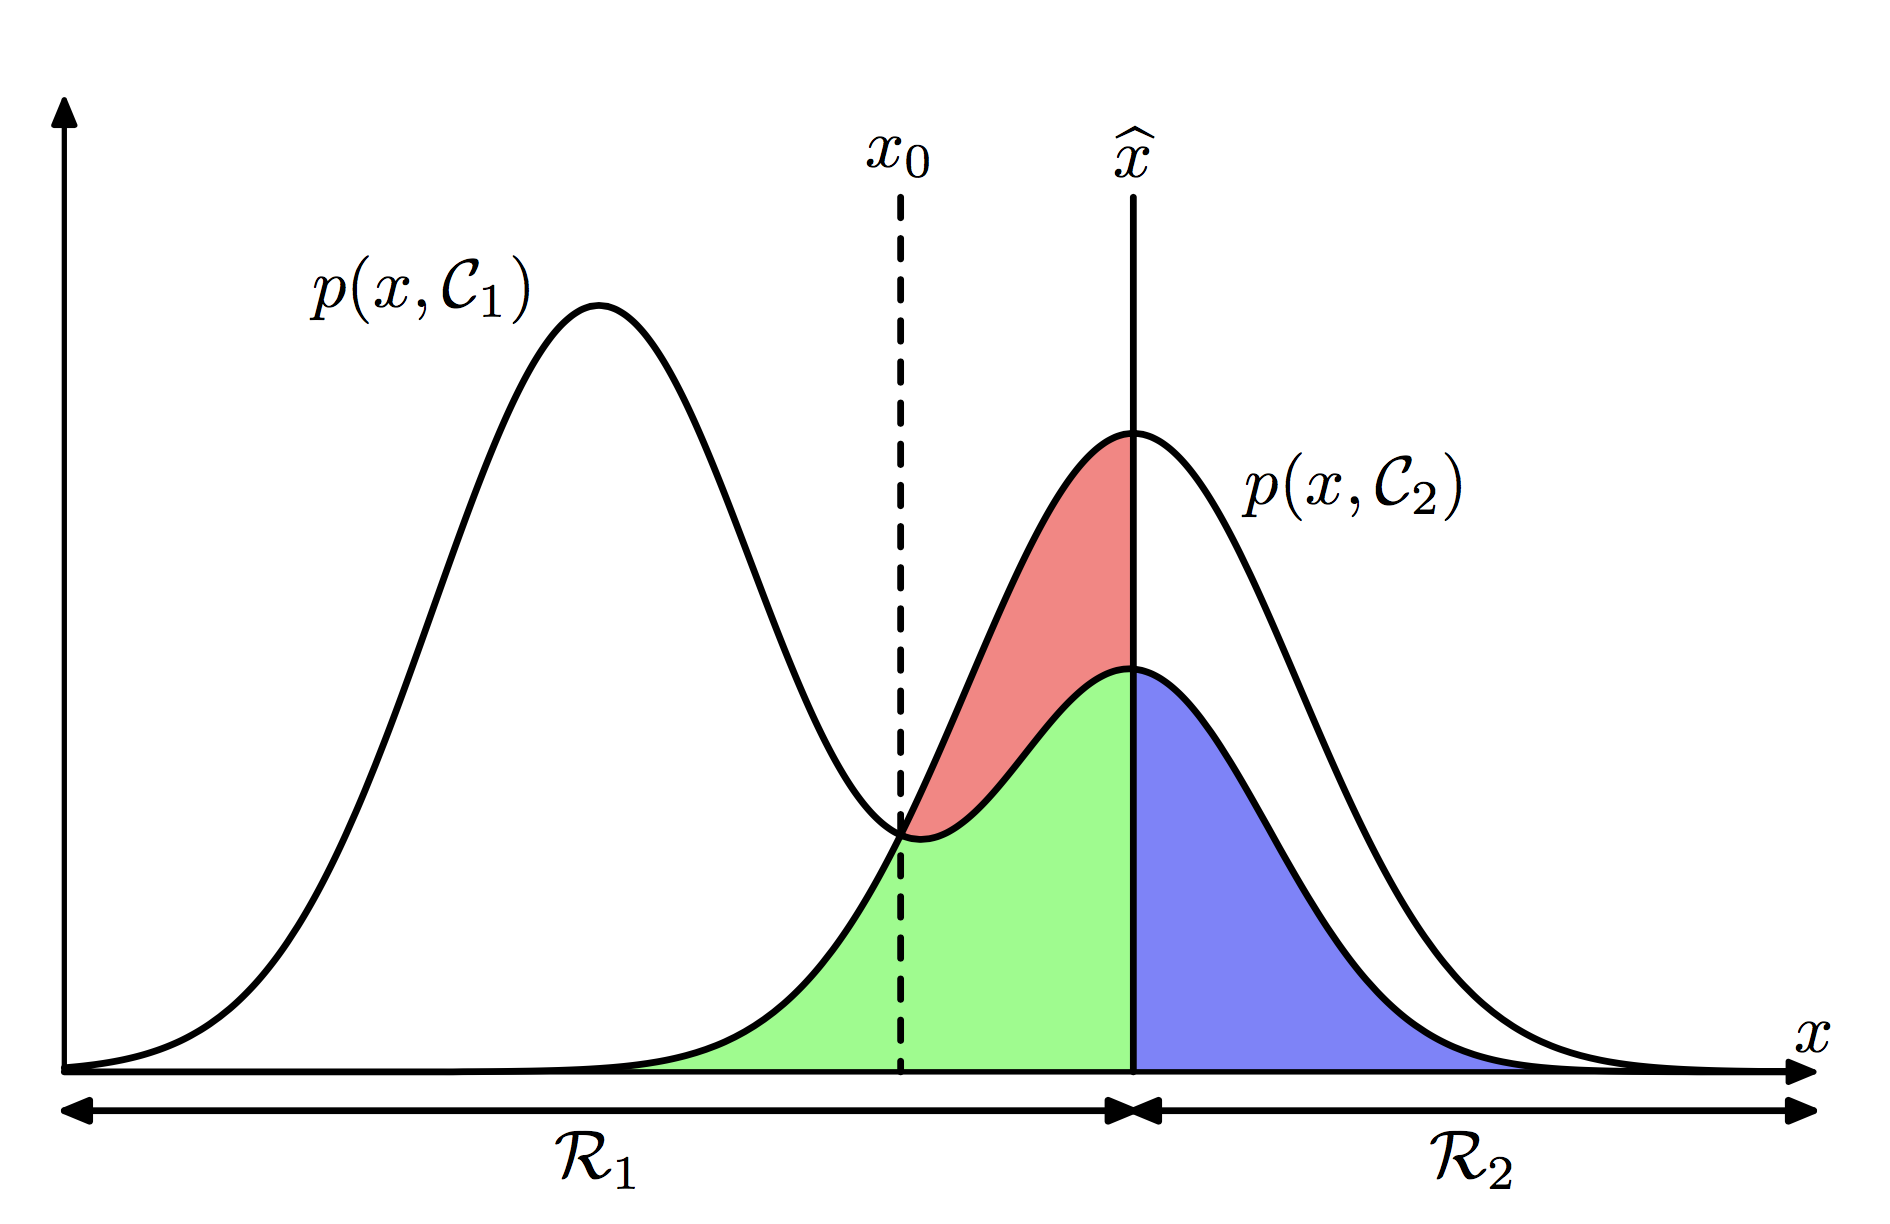
\includegraphics[scale=0.17]{classification_joint_dist.png}
    \caption{
      Schematic illustration of the joint probability distribution $p(x,\mathcal{C}_k)$.
    }
    \end{figure}

    Our goal in decision stage is to make a decision to minimize the $\mathit{loss\ function}$
    given a new input $x$ based on the probabilistic representation. The loss
    function may be denoted in several ways as follows:
    \begin{equation}
      \textrm{loss\ function}: \quad L(t, \hat{t})
             \quad \textrm{or} \quad L(t, x)
             \quad \textrm{or} \quad L(t, y(x))
    \end{equation}
    At these notations, $t$ is the true target value corresponding to $x$, and
    $\hat{t}$ is the decision based on a specific rule $y$ given the new
    observation $x$, so that the function $L$ is a single, overall measure of
    loss incured in taking the decision $\hat{t}$ but the true value being $t$
    given $x$. Let's look at two examples to help you understand.
  \end{justify}
\end{frame}

\begin{frame}{Loss Function (conti\ldots)}
  \begin{justify}
    \textbf{e.g.\ classification problem}\\
    In classification problem, we should classify $x \in S$ into some class
    $\mathcal{C}_k \, \forall k \in \{ 1,\ldots,K \}$. Let a rule $\mathcal{R}_k$
    be the subset of $S$ and the rule assigns all points $x \in \mathcal{R}_k$
    into $\mathcal{C}_k$, then we can define the loss function as follows:
    \begin{equation}
       \forall k,j \in \{ 1,\ldots,K \}; \quad
       L(t, x) = L(\mathcal{C}_{k}, x \in \mathcal{R}_j)
        = \left\{\begin{aligned}
          & 0       \quad && (k = j)  \\
          & L_{kj}  \quad && (k \neq j)
        \end{aligned}\right.
    \end{equation}
    And we may also represent this function in matrix form, which is called
    $\mathit{loss\ matrix}$.
    \begin{equation}
      \mathbfit{L}
        = \left\{\begin{aligned}
          & 0       \quad && (i = j)  \\
          & L_{kj}  \quad && (i \neq j)
        \end{aligned}\right.
    \end{equation}

    \vspace{0.5\baselineskip}
    \textbf{e.g.\ regression problem}\\
    In regression problem, we should find some value $\hat{t}$ based on a specific
    rule $y$ given the new observation $x \in S$. The loss incurred in making decision
    based on rule $y$ can be defined as follows:
    \begin{equation}
      L(t, y(x))
    \end{equation}
    in some cases, we can use square term or absolute value term:
    \begin{equation}
      L(t, y(x)) = |t-y(x)| \quad \textrm{or} \quad {(t-y(x))}^2
    \end{equation}
  \end{justify}
\end{frame}

\begin{frame}{Minimizing Expected Loss}
  \begin{justify}

    In the classification example, the optimal solution is the one which minimizes
    the loss function. However, the loss function depends on the true class $\mathcal{C}_k$,
    which is unknown. For a given input $x$, our uncertainty in the true class
    is expressed through the joint probability distribution $p(x, \mathcal{C}_k)$, which
    is evaluated through inference stage, and so we seek instead to minimize the
    average loss, where the average is computed with respect to this distribution,
    which is given by
    \begin{equation}
      \begin{split}
        \mathbb{E}[L]
          &= \sum_k \sum_j \int_{\mathcal{R}_j} L_{kj} p(x, \mathcal{C}_k)\, \mathrm{dx} \\
          &= \sum_j \int_{\mathcal{R}_j} \sum_k \{L_{kj} p(x, \mathcal{C}_k)\}\, \mathrm{dx}
      \end{split}
    \end{equation}
    Now, our goal is to choose the rule $\mathcal{R}_j$ which minimize
    $\sum_k \{L_{kj} p(x, \mathcal{C}_k)\}$ for each $x$. And we may use the
    product rule  $p(x,\mathcal{C}_k) = p(\mathcal{C}_k|x)p(x)$ to eliminate
    the common factor of $p(x)$, then we get:
    \begin{equation}
      x \in \mathcal{R}_{j^*} \quad \textrm{s.t.} \quad j^*
      = \argmin_j \sum_k \{L_{kj} p(x, \mathcal{C}_k)\}
      = \argmin_j \sum_k \{L_{kj} p(\mathcal{C}_k | x)\}
    \end{equation}
    where $p(\mathcal{C}_k, x)$ is the posterior. Hence, it is clear that the
    decision rule that minimizes the expected loss is the one that assigns each
    new $x$ to the class $j$ to minimize (58).
  \end{justify}
\end{frame}

\begin{frame}{Reject Option}
  \begin{columns}
    \begin{column}{0.3\textwidth}
      \begin{figure}
      \centering
      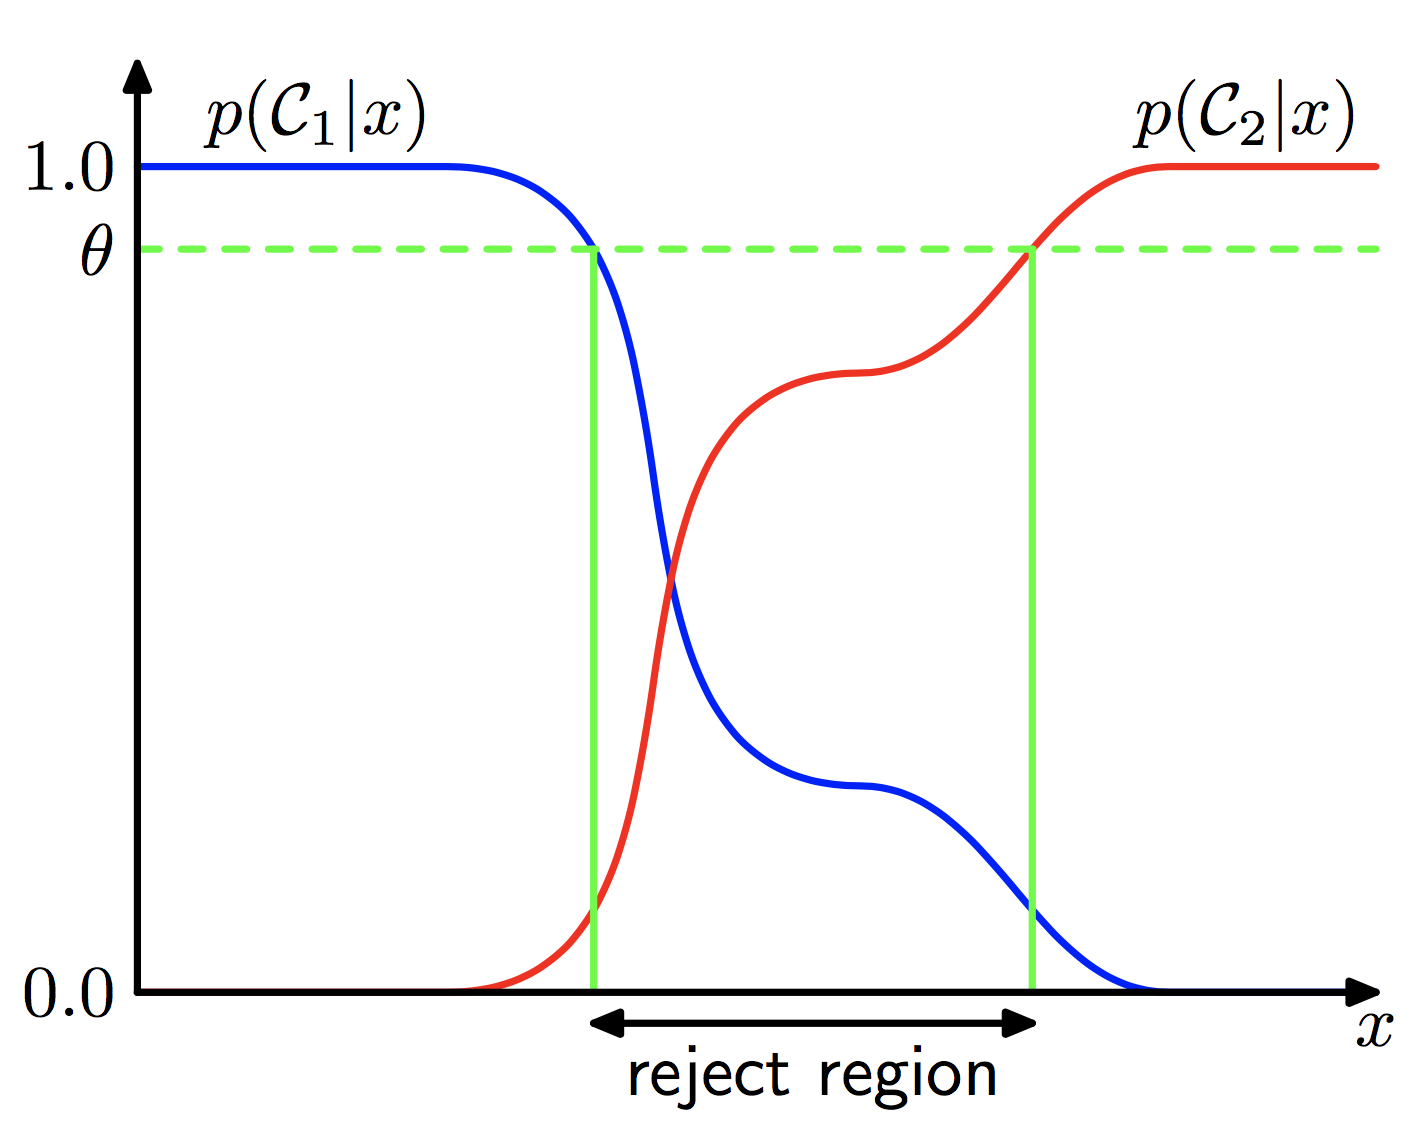
\includegraphics[scale=0.15]{classification_rejection_option.png}
      \caption{
        Schematic illustration of the joint probability distribution $p(x,\mathcal{C}_k)$.
      }
      \end{figure}
    \end{column}
    \begin{column}{0.7\textwidth}
      \begin{justify}
        In some cases, the largest of the posterior probabilities $p(\mathcal{C}_k|x)$
        is significantly less than unity,
        \begin{equation}
          \frac{p(\mathcal{C}_k|x)}{\sum_{k} p(\mathcal{C}_k|x)} << 1
        \end{equation}
        or equivalently, the joint distribution $p(x,\mathcal{C}_k)$ have comparable values.
        For these cases where the optimal decision is not significantly superior to
        the alternative, it is relatively uncertain which class the value x is assigned to.
        Hence, in some applications, it will be appropriate to avoid making decisions
        on the difficult cases in anticipation of a lower error rate on those examples
        for which a classification decision is made. This is known as the
        $\mathit{rejection\ option}$.
        \begin{equation}
          \frac{\max_k p(\mathcal{C}_k|x)}{\sum_{k} p(\mathcal{C}_k|x)} \ll \theta
          \quad \mathrm{where} \quad \frac{1}{k} \leq \theta \leq 1
        \end{equation}
      \end{justify}
    \end{column}
  \end{columns}
\end{frame}

\subsection{Inference stage}
\begin{frame}{Gen or Dis}
  \begin{justify}
    Now, step back and see the big picture, ``the whole process of machine learning.''
    We have been divide the machin learning process into two sub stages, inference
    step in which we use training data to learn a probabilistic model, says, $p(t|x)$,
    and decision step in which we use these probabilistic representation to make
    optimal decision. There is an ambiguity arises, how to learn probabilistic
    model, and what it looks like? Furthermore, we may consider the case where
    do not use probabilistic inference.

    In fact, we can identify three distinct approaches to solving decision problems,
    all of which have been used in practical applications.

    \vspace{0.5\baselineskip}
    \textbf{Generative Method}\\
    models how the data was generated in order to categorize a signal. It asks
    the question: based on my generation assumptions, which category is most
    likely to generate this signal?\\

    \vspace{0.5\baselineskip}
    \textbf{Discriminative Method}\\
    A discriminative algorithm does not care about how the data was generated,
    it simply categorizes a given signal. This category can be subdivided again
    into two subcategories:\\

    \begin{itemize}
      \item\begin{justify}
        \textbf{Probabilistic Discriminative Method} is a stochastic way,
        which may directly model $p(t|x)$ (e.g.\ logistic regression).
      \end{justify}
      \item\begin{justify}
        \textbf{Deterministic Discriminative Method} is a non-stochastic way,
        which directly find function that directly maps $x$ to target value $t$
        without any statistical inference.
      \end{justify}
    \end{itemize}
  \end{justify}
\end{frame}

\begin{frame}{Gen or Dis (cont\ldots)}
  \begin{justify}
    Now for your understanding, let's re-visit the classification problem.
    \vspace{0.5\baselineskip}
    \textbf{Generative} \\
      \begin{enumerate}
        \item Solve the inference problem of determining the class-conditional
              densities $p(x|\mathcal{C}_k)$ for each class $\mathcal{C}_k$ individually.
        \item Separately infer the prior $p(\mathcal{C}_k)$.
        \item Use Bayes' theorem to find the posterior $p(\mathcal{C}_k|x)$.
        \item Equivalently, we can model the joint distribution $p(x,\mathcal{C}_k)$
              directly and then normalize to obtain the posterior $p(\mathcal{C}_k)$.
        \item Having found the posterior $p(\mathcal{C}_k)$, we use decision theory
              to determine class membership for each new input $x$.
      \end{enumerate}

    \vspace{0.5\baselineskip}
    \textbf{Probabilistic Discriminative} \\
      \begin{enumerate}
        \item First solve the inference problem of determining the posterior $p(\mathcal{C}_k|x)$,
        \item And then, use decision theory to assign each new $x$ to one of the classes.
      \end{enumerate}

    \vspace{0.5\baselineskip}
    \textbf{Deterministic Discriminative} \\
      \begin{enumerate}
        \item Find a function $f(x)$, called a discriminant function, which maps
              each input $x$ directly onto a class label.
      \end{enumerate}
  \end{justify}
\end{frame}

\begin{frame}{Usefulness of Posterior}
  \begin{justify}
    Although the stochastic inference stage requires much more cost, we will use
    them since there are many powerful reasons for wanting to compute the posterior.

    \vspace{0.5\baselineskip}
    \textbf{Minimizing Risk}
    \begin{equation}
      x \in \mathcal{R}_{j^*} \quad \textrm{s.t.} \quad j^*
      = \argmin_j \sum_k \{L_{kj} p(\mathcal{C}_k | x)\}
    \end{equation}

    \textbf{Reject Option}
    \begin{equation}
      \frac{\max_k p(\mathcal{C}_k|x)}{\sum_{k} p(\mathcal{C}_k|x)} \ll \theta
    \end{equation}

    \textbf{Compensating for class priors} \\
    sometimes we need to modify a data set to adjust an innate rarity of a specific
    event, such as cancer.
    \begin{equation}
        \textrm{True prior:}\: p(\mathcal{C}_k),\,
        \textrm{Balanced posterior:}\: q(\mathcal{C}_k|x) \propto q(x|\mathcal{C}_k) q(\mathcal{C}_k)
    \end{equation}
    Although the balanced dataset would allow us to find a more accurate model, we
    then have to compensate for the effects of our modifications to the training data.
    \begin{equation}
      \textrm{Adjusted posterior:} \quad \tilde{p}(\mathcal{C}_k|x) \propto q(\mathcal{C}_k|x) \frac{p(\mathcal{C}_k)}{q(\mathcal{C}_k)}
    \end{equation}
  \end{justify}
\end{frame}

\begin{frame}{Usefulness of Posterior (conti\ldots)}
  \begin{justify}
    \textbf{Combining models}\\
    For complex applications, we may wish to break the problem into a number of
    smaller subproblems each of which can be tackled by a separate module. In
    some cases where more than a type of data is available, rather than combine
    all of this heterogeneous information into one huge input space, it may be
    more effective to build more than one system to interprete each type of data.

    \vspace{0.5\baselineskip}
    One simple way to do this is to assume that, for each class separately, the
    distributions of inputs, denoted by $x_1$ and $x_2$, are independent, so that
    \begin{equation}
        P(x_1, x_2|\mathcal{C}_k) = P(x_1 | \mathcal{C}_k) P(x_2|\mathcal{C}_k)
        \quad \textrm{where} \quad x_1 \perp x_2 \,|\, \mathcal{C}_k
    \end{equation}

    The posterior is then given by
    \begin{equation}
      \begin{split}
        P(\mathcal{C}_k|x_1, x_2)
          & \propto p(x_1|\mathcal{C}_k) p(x_2|\mathcal{C}_k) p(\mathcal{C}_k) \\
          & \propto \frac{p(\mathcal{C}_k|x_1) p(\mathcal{C}_k|x_2)}{p(\mathcal{C}_k)}
      \end{split}
    \end{equation}
  \end{justify}
\end{frame}

%%%%%%%%%%%%%%%%%%%%%%%%%%%%%%%%%%%%%%%%%%%%%%%%%%%%%%%%%%%%%%%%%%%%%

\section{Information Theory}
\subsection{Probability and Information}
\begin{frame}{Self Information}
  \begin{justify}
    \textbf{Principle of quantifying Information} \\

    \begin{enumerate}
      \item Likely events should have low information content. Less likely events
            should have higher information content.
      \item Independent events should have additive information.
    \end{enumerate}

    \textbf{Self-information} \\
    By above principle, we can define self-information like:
    \begin{equation}
      h(x) = - \ln P(x)
    \end{equation}

    \textbf{Shannon Entropy} \\
    We can quantify uncertainty of whole distribution like:
    \begin{equation}
      H[x] = \mathbb{E}_{x \sim P} [I(x)] = -\mathbb{E}_{x \sim P} [\ln P(x)]
    \end{equation}
    Shonnon entrophy means expected amount of information in an event drawn
    from that distribution.

  \end{justify}
\end{frame}

%\begin{frame}{Others\ldots}
%\end{frame}

\subsection{Entrophy}
\begin{frame}{Entrophy (discrete)}
  \begin{justify}
    \textbf{Kullbeck-Leibler(KL) Divergence}\\
    We sometimes want to know how different two distributions are. In this case,
    we use KL divergence defined by:
    \begin{equation}
      KL(P||Q) = \mathbb{E}_{x \sim P}[\ln \frac{P(x)}{Q(x)}] = \mathbb{E}_{x \sim P}[\ln P(x) - \ln Q(x)]
    \end{equation}

    And it means extra amount of information needed to send a message containing
    symbols drawn from probability distribution P, when we use a code that was
    designed to minimize the length of messages drawn from probability distribution.

    \textbf{Cross-Entrophy}~\cite{Goodfellow-et-al-2016}\\
    Cross-entrophy which means the average number of information needed to encode
    data coming from a source with distribution P when we use model q to define our
    codebook. (not extra)

    \vspace{0.5\baselineskip}
    We can define cross-entrophy like:
    \begin{equation}
      H(P,Q) = H(P) + KL(P||Q) = -\mathbb{E}_{x \sim P}[\ln Q(x)]
    \end{equation}
  \end{justify}
\end{frame}

%\begin{frame}{Maximum entrophy (discrete)}
%\end{frame}

%\begin{frame}{Differentail entrophy (continuous)}
%\end{frame}

%\begin{frame}{Maximum entrophy (continuous)}
%\end{frame}

% \subsection{Comparison between two distributions}
% \begin{frame}{Kullbeck-Leibler Divergence}
%   \begin{itemize}
%     \item Kullbeck-Leibler (KL) Divergence
%     \item Cross Entrophy
%   \end{itemize}
% \end{frame}

%\begin{frame}{KL Divergence (conti\ldots)}
%\end{frame}
%%%%%%%%%%%%%%%%%%%%%%%%%%%%%%%%%%%%%%%%%%%%%%%%%%%%%%%%%%%%%%%%%%%%%
\printbibliography\subsection{References}
\end{document}
%%%%%%%%%%%%%%%%%%%%%%%%%%%%%%%%%%%%%%%%%%%%%%%% DOCUMENT start
